\chapter{Automatische Redeneersystemen}
\label{s:automaticReasoning}
\chapterquote{Logica is de architectuur van de menselijke rede.}{Evelyn Waugh, Brits schrijfster (1903-1966)}
Naast zoekproblemen en het oplossen van constraint netwerken, blijkt de Artifici\"ele intelligentie ook een uiterst geschikt domein te zijn voor logica. Al in de jaren '60 had men het droombeeld van de computer als stellingbewijzer. Met logica kan immers alles formeel uitgedrukt worden. Bijgevolg, zo redeneerde men, kan men een machine bouwen die door het toepassen van simpele regels, in staat moet zijn om met een stelsel uitspraken, een afgeleide uitspraak te kunnen bewijzen. Deze hypothese is werd gestaafd met volgende argumenten:
\begin{itemize}
 \item Logica is de assembleertaal van de kennis en ligt bovendien heel dicht bij de natuurlijke taal: bijgevolg kan men bijna elke vorm van kennis omzetten in formele ondubbelzinnige logica.
 \item Als computers kennis moeten verwerken, dan moet die kennis formeel en ondubbelzinnig zijn.
 \item Door middel van \termen{Logische Deductie} moeten we op een systematische manier nieuwe kennis uit bestaande kennis kunnen synthetiseren.
\end{itemize}
De vraag is dus of we deze deductie kunnen automatiseren.
\section{Leidend voorbeeld: Marcus Brutus}
\begin{leftbar}
Stel we beschikken over volgende bestaande kennis:
\begin{enumerate}
 \item Marcus was een man
 \item Marcus was een Pompei\"er
 \item Alle Pompei\"ers waren Romeinen
 \item Cesar was een Heerser
 \item Alle Romeinen waren ofwel loyaal aan Cesar of probeerden hem te vermoorden
 \item Iedereen is loyaal aan iemand
 \item Mensen proberen alleen heersers te vermoorden waar ze niet loyaal aan zijn
 \item Marcus probeerde Cesar te vermoorden
 \item Iedere man is een mens.
\end{enumerate}
We willen een antwoord vinden op de vraag ``Was Marcus  Loyaal aan Cesar?''. Indien we dit zelf uitwerken zullen we meestal eerst alle uitspraken omzetten naar \termen{Eerste Orde logica}:
\begin{enumerate}
 \item $\mathfunc{man}{\Marcus}$
 \item $\mathfunc{pompei\"er}{\Marcus}$
 \item $\forall x:\mathfunc{pompei\"er}{x}\rightarrow\mathfunc{romein}{x}$
 \item $\mathfunc{heerser}{\Cesar}$
\item $\forall x:\mathfunc{romein}{x}\rightarrow\left(\begin{array}{c}\mathfunc{loyaalAan}{x,\Cesar}\wedge\neg\mathfunc{probeerTeVermoorden}{x,\Cesar}\\\vee\\\neg\mathfunc{loyaalAan}{x,\Cesar}\wedge\mathfunc{probeerTeVermoorden}{x,\Cesar}\end{array}\right)$
 \item $\forall x, \exists y:\mathfunc{loyaalAan}{x,y}$
 \item $\forall x,y:\mathfunc{mens}{x}\wedge\mathfunc{heerser}{y}\wedge\mathfunc{probeerTeVermoorden}{x,y}\rightarrow\neg\mathfunc{loyaalAan}{x,y}$
 \item $\mathfunc{probeerTeVermoorden}{\Marcus,\Cesar}$
 \item $\forall x:\mathfunc{man}{x}\rightarrow\mathfunc{mens}{x}$
\end{enumerate}
We proberen dan te bewijzen dat Marcus loyaal was aan Cesar, of formeler $\mathfunc{loyaalAan}{\Marcus,\Cesar}$. Anderzijds kunnen we ook door middel van \termen{Achterwaarts redeneren} proberen te bewijzen dat Marcus niet loyaal is aan Cesar en tot een inconsistentie trachtten te komen. Indien we $\neg\mathfunc{loyaalAan}{\Marcus,\Cesar}$ als beginexpressie kiezen, kunnen we een substitutie uitvoeren met behulp van 7. Hierbij vervangen we $x$ door $\Marcus$ en $y$ door $\Cesar$. Vervolgens bekomen we $\mathfunc{mens}{\Marcus}\wedge\mathfunc{heerser}{\Cesar}\wedge\mathfunc{probeerTeVermoorden}{\Marcus,\Cesar}\rightarrow\neg\mathfunc{loyaalAan}{\Marcus,\Cesar}$. Indien we deze drie componenten kunnen aantonen kunnen we bewijzen, hebben we meteen bewezen dat Marcus niet loyaal is aan Cesar. Aangezien 9 geldt en we weten door 1 dat Marcus een man is, kunnen we het eerste statement vervangen door $\mathfunc{man}{\Marcus}$. Aangezien dit laatste een feit is (door 1), en de twee andere aspecten in de vergelijking ook feiten zijn (door 4 en 8). Kunnen we vervolgens bewijzen dat Marcus niet loyaal was aan Cesar. Schematisch wordt dit bewijs ook getoond op figuur \ref{fig:proofMarcusCesar}.
\end{leftbar}
\begin{figure}[htb]
\centering
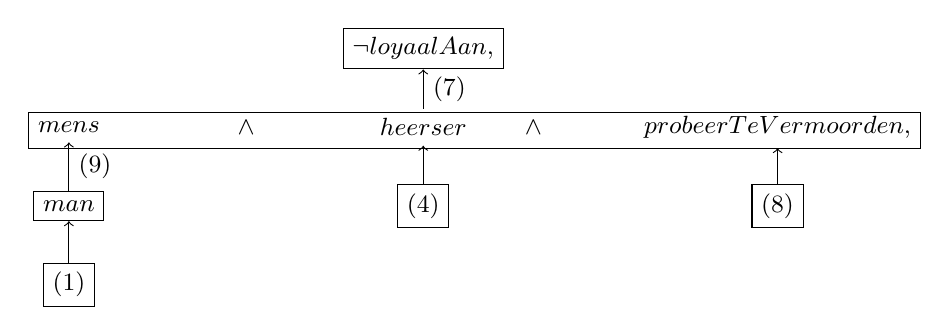
\begin{tikzpicture}
\def\dy{-1cm};
\def\dx{4.5cm};
\node[draw=black,rectangle] (S1) at (0,0) {\small{$\neg\mathfunc{loyaalAan}{\Marcus,\Cesar}$}};
\node (S2a) at (-\dx,\dy) {\small{$\mathfunc{mens}{\Marcus}$}};
\node (S2b) at (0,\dy) {\small{$\mathfunc{heerser}{\Cesar}$}};
\node (S2c) at (\dx,\dy) {\small{$\mathfunc{probeerTeVermoorden}{\Marcus,\Cesar}$}};
\draw (S2a.north west) rectangle (S2c.south east);
\node (S2ma) at (-2.25 cm,\dy) {\small{$\wedge$}};
\node (S2mb) at (1.4 cm,\dy) {\small{$\wedge$}};
\draw[->] (S2b) to node[midway,anchor=west]{\small{$(7)$}} (S1);
\node[draw=black,rectangle] (S3a) at (-\dx,2*\dy) {\small{$\mathfunc{man}{\Marcus}$}};
\node[draw=black,rectangle] (S3b) at (0,2*\dy) {\small{$(4)$}};
\node[draw=black,rectangle] (S3c) at (\dx,2*\dy) {\small{$(8)$}};
\draw[->] (S3a) to node[midway,anchor=west]{\small{$(9)$}} (S2a);
\draw[->] (S3b) -- (S2b);
\draw[->] (S3c) -- (S2c);
\node[draw=black,rectangle] (S4a) at (-\dx,3*\dy) {\small{$(1)$}};
\draw[->] (S4a) -- (S3a);
\end{tikzpicture}
\caption{Bewijs voor disloyaliteit van Marcus jegens Cesar}
\label{fig:proofMarcusCesar}
\end{figure}
\paragraph{}
Bovenstaand voorbeeld legt echter onmiddellijk een paar problemen bloot:
\begin{enumerate}
 \item Kennisrepresentatie:
\begin{enumerate}
 \item Imprecies taalgebruik: niet alle taal is machinaal onmiddellijk te vervangen door logica (bijvoorbeeld 7)
 \item Evidente informatie: vooral 9 wordt bijvoorbeeld makkelijk vergeten omdat deze vanzelfsprekend is
 \item Niet alle informatie is makkelijk voor te stellen met logica (zoals ``bijna'',``meestal'',...)
 \item Logica is niet handig vanuit ``Sofware-engineering'' perspectief (lijkt te veel op assembler)
\end{enumerate}
 \item Problem solving:
\begin{enumerate}
 \item Een groot aantal tradeoffs die ook bij zoekmethodes voorkwamen (zie \ref{ss:stateSpaceTradeOffs})
 \item Welke deductieregels hebben we nodig (Modus Ponens, Modus Tollens,...)
 \item Hoe behandelen we $\forall x$ en $\exists y$
 \item Hoe berekenen we substituties (in het voorbeeld eenvoudig, in de praktijk soms oneindig veel mogelijkheden)
 \item Wat bewijzen we? ``Het te bewijzen'' of het omgekeerde?
 \item Hoe behandelen we gelijkheid van statements (twee verschillende expressies kunnen soms wel equivalent zijn, door symmetrie, reflexiviteit, transitiviteit)
 \item Hoe garanderen we de volledigheid en de correctheid?
\end{enumerate}
\end{enumerate}
\section{De formele model semantiek van Logica}
Alvorens al die problemen op te lossen is het zinvol eerst opnieuw stil te staan bij het wiskundige concept van logica. Deze subsectie mag dan ook overgeslagen worden indien de propositie- en predicatenlogica reeds in andere cursussen behandeld werd.
\subsection{Propositielogica}
In propositielogica zijn we in staat simpele expressies voor te stellen door middel van een beperkt \termen{alfabet} (reeks toegelaten karakters). Dit alfabet kunnen we onderverdelen in drie subsets:
\begin{itemize}
 \item \termen{Atomaire Proposities}: Dit zijn expressies waar we een bepaalde eigenschap aan geven. Hun namen worden door de gebruiker zelf gekozen (bijvoorbeeld $\left\{\mbox{weer\_is\_regenachtig},\mbox{Jos\_draagt\_paraplu}\right\}$)
 \item \termen{Connectieven}: Om atomaire proposities met elkaar te combineren gebruiken we connectieven. Deze set staat vast en bevat volgende elementen: $\left\{\wedge,\vee,\neg,\rightarrow,\leftarrow,\leftrightarrow\right\}$
 \item \termen{Punctuaties}: Bij connectieven gelden bepaalde voorrangsregels, om deze aan te passen beschikken we over punctuaties of haakjes, deze set staat vast en bevat volgende elemententen: $\left\{(,)\right\}$
\end{itemize}
Een \termen{Goed Gevormde Formule} in de propositielogica is een expressie die enkel gebruik maakt van het alfabet van de propositielogica, en daarbij de regels respecteert van de connectieven en de punctuaties.
\begin{leftbar}
Hieronder worden enkele concrete schoolvoorbeelden van propositielogica weergegeven:
\begin{equation}
\left\{\begin{array}{l}
\mbox{afstandsbediening\_is\_kapot}\vee\neg\mbox{tv\_werkt}\\
\mbox{schilderij\_is\_gestolen}\rightarrow\neg\mbox{schilderij\_hangt\_hier}\\
\mbox{Gabriela\_tennist}\wedge\mbox{Judith\_schaakt}\\
\mbox{er\_loopt\_stroom}\rightarrow\mbox{draad\_wordt\_warm}\\
\mbox{Jos\_draagt\_paraplu}\leftarrow\mbox{weer\_is\_regenachtig}
\end{array}\right.
\end{equation}
\end{leftbar}
\paragraph{Semantiek}
We kunnen de betekenis of \termen{semantiek} van een expressie vastleggen op twee manieren: Door middel van natuurlijke taal, of door middel van \termen{transformationele semantiek}. In dat laatste geval beschrijven we de statements door een daar uit afgeleid mathematisch object. Zo kunnen we bijvoorbeeld uit een reeks statements alle atomaire proposities die waar zijn doormiddel van \termen{logisch gevolg} weergeven. Indien we vervolgens een expressie controleren kunnen we deze opbouwen vanuit de waarheidstabel.
\paragraph{Logisch Gevolg}
Maar hoe defini\"eren we dan logisch gevolg? intu\"itief denken we aan alles wat we logisch gezien willen vastleggen maar dit is niet het geval. Op dit ogenblik hebben we immers nog geen verzameling afleidingsregels. Dat is immers wat we willen vastleggen! Een logisch gevolg wordt bereikt door \termen{Interpretatie} en een \termen{Model}:
\begin{description}
 \item[Interpretatie:]Is een functie die aan iedere atomaire formule een bepaalde waarheidswaarde toekent, en vervolgens alle statements coontroleert. We genereren dus een \termen{waarheidstabel}.
 \item[Model:]Een model toetst vervolgens deze statements op hun waarheid. Configuraties waarbij geen statements falen worden hierbij als een logisch gevolg gezien. Een model $M$ is dus een subset van een interpretatie $I$ indien alle expressies waarop de expressie gebaseerd zijn, waar zijn.
\end{description}
Of meer formeel: Gegeven een stel formules (statements) $S$ en een formule $F$. $F$ is een logisch gevolg van $S$ ($S\vDash F$) indien elk model van $S$ ook $F$ waarmaakt.
\subsection{Predicatenlogica}
Hoewel propositielogica reeds heel wat problemen kan oplossen, kunnen we het leidende voorbeeld er niet in uitdrukken. Hiervoor hebben we een algemenere taal nodig, de \termen{predicatenlogica}. Het alfabet van de predicatenlogica bestaat uit de volgende elementen:
\begin{itemize}
 \item \termen{Variabelen} (zoals $x$ en $y$): deze vervullen een tijdelijke rol met behulp van kwantoren
 \item \termen{Constanten} (zoals $\Cesar$ en $\Marcus$): hun rol is globaal en dus gedefinieerd over alle statements
 \item \termen{Functie-symbolen} (zoals $\mbox{vader}$, $\mbox{hart}$,...): om bepaalde relaties ten opzichte van variabelen en constanten te defini\"eren
 \item \termen{Predicaatsymbolen} (zoals $\mbox{mens}$, $\mbox{loyaalAan}$,...): gebruikers gedefinieerde symbolen om een algoritme te kunnen laten werken, deze kennen bovendien een waarheidswaarde toe.
 \item Connectieven ($\wedge$, $\neg$,...): om meer geavanceerde uitspraken te doen (net als bij propositielogica)
 \item Punctuaties ($($ en $)$): het geven van prioriteit aan een bepaald deel van de expressie
 \item \termen{Quantoren} ($\forall$ en $\exists$): het geven van een invulling aan de variabelen
\end{itemize}
Verder introduceren we nog een nieuw concept in de predicatenlogica: Een \termen{term}. Een term is een variabele, een constante of een functiesymbool voorzien van met termen (wat cascadering van functies mogelijk maakt) zoveel als het verwachtte aantal voor de functie. Concrete voorbeelden zijn $\mathfunc{moordenaar}{\Cesar}$, $\mathfunc{dochter}{x,\Cesar}$ en $\mathfunc{hart}{\mathfunc{vader}{\Marcus}}$. Een goed-gevormde formule in predicatenlogica wordt geconstrueerd uit predicaat-symbolen voorzien met termen als argumenten en uit connectoren, quantoren en punctuaties, en dit volgens de regels die connectoren opleggen.
\paragraph{}
Een Goed Gevormde Formule in predicatenlogica is een expressie die zich tot het alfabet van de predicatenlogica beperkt, en daarnaast de regels voor connectieven en punctiaties respecteren, verder bevatten ze geen variabelen die niet door een quantor gedefinieerd zijn (in de expressie zelf).
Hoe moeten we nu deze formules interpreteren? We kunnen een expressie in predicatenlogica zien als een combinatie van enkele factoren:
\begin{itemize}
 \item Een verzameling $D$ die we het domein noemen waarin alle constanten zitten.
 \item De Functie-symbolen als wiskundige functies die van $D\rightarrow D$ gedefinieerd zijn
 \item De predicaatsymbolen als wiskundige functies die van $D\rightarrow\Bb$ gedefinieerd zijn ($\Bb=\left\{\true,\false\right\}$ is de verzameling booleans)
 \item De quantoren op variabelen lezen we als volgt:
\begin{itemize}
 \item $\forall x\ f\left(x\right)$ is waar indien $\forall d\in D:I\left(f\left(d\right)\right)=\true$ (hierbij is $I$ de identiteitsfunctie die $\true$ op $\true$ en $\false$ op $\false$ afbeeldt)
 \item $\exists x\ f\left(x\right)$ is waar indien $\exists d\in D:I\left(f\left(d\right)\right)=\true$
\end{itemize}
\end{itemize}
\section{Automatisch Redeneer-systemen voor eerste-orde predicatenlogica}
In deze subsectie zullen we een automatisch rendeneer-systeem voor eerste-orde predicaten logica ontwerpen. Hierbij bezitten we een kennisbank geschreven in predicatenlogica die we $T$ noemen. Dit is een verzameling van eerste-orde formules en wordt formeel ook wel eens de ``\termen{Theorie}'' genoemd. Verder beschikken we over een bijkomende eerste-orde predicatenlogica-formule $F$. De vraag die beantwoordt dient te worden is of $T$, $F$ impliceert, of formeler: $T\vDash F$. We zoeken dus een afleidingstechniek die dit kan uitmaken voor iedere $F$ en $T$. Daarnaast zijn ook correctheid, volledigheid en efficientie vereiste criteria.
\subsection{Beslisbaarheid}
Is iedere formule te beslissen? Volgens de \termen{stelling van Church}, bestaat er geen enkel algoritme dat in staat is voor iedere $T$ en $F$ uit te maken of $T\vDash F$. Dit ondermijnt dus onmiddellijk ons eerder gestelde doel: Niet elk probleem is beslisbaar. Anderzijds zegt de \termen{Volledigheidsstelling van G\"odel} dat er een redeneertechniek bestaat waarbij voor iedere $T$ en $F$ waarbij $T\vDash F$, deze techniek dit kan bewijzen. Dit wordt \termen{semi-beslisbaarheid} genoemd. Dus indien $F$ uit $T$ volgt, is dit bewijsbaar. Indien we noch $T\vDash F$ noch $T\vDash \neg F$ kunnen bewijzen, kunnen we bijgevolg niets zeggen over $F$.
\subsection{Achterwaartse Resolutie}
In het algemeen wordt voor automatisch redeneren in de eerste orde slechts \'e\'en aanpak gehanteerd: \termen{Achterwaartse resolutie}. Deze techniek bevat verschillende technische componenten, die we stap voor stap zullen uitwerken, en waarbij we de predicatentaal zullen uitbreiden van \termen{Gegronde Horn Clause Logica} over \termen{Horn Clause logica} en \termen{Clausale logica} tot uiteindelijk de volledige predicatenlogica. Voor elk van deze talen zullen we een semi-beslisbare procedure bouwen, die we verder zullen moeten verfijnen indien we de taal uitbreiden. De achterwaartse resolutie is gebaseerd op de volgende principes:
\begin{itemize}
 \item \termen{Clausale vorm} (in \ref{sss:clausaleLogic} op pagina \pageref{sss:clausaleLogic})
 \item \termen{Bewijs door inconsistentie} (in \ref{sss:inconsistenceProof} op pagina \pageref{sss:inconsistenceProof})
 \item \termen{Unificatie} (in \ref{sss:unification} op pagina \pageref{sss:unification})
 \item De \termen{Resolutie stap} (in \ref{sss:resolutionStep} op pagina \pageref{sss:resolutionStep})
 \item De \termen{Resolutie bewijzen} (in \ref{sss:resolutionProof} op pagina \pageref{sss:resolutionProof})
 \item \termen{Normalisatie} (in \ref{sss:normalisation} op pagina \pageref{sss:normalisation})
\end{itemize}
Nadat we eerst de verschillende beperkte predicaattalen uitleggen in subsubsecties \ref{sss:gegrondeHornClausaleLogic}, \ref{sss:hornClausaleLogic} en \ref{sss:clausaleLogic}, worden
deze principes in de  verdere subsubsecties verder uitgelegd. Na een korte introductie zal vervolgens dieper ingegaan op de materie. Eventueel kan de lezer bij ieder item eerst de eerste paragraaf lezen, en vervolgens zijn kennis uitbreiden met de overige paragrafen.
\subsection{Gegronde Horn Clause Logica}
\label{sss:gegrondeHornClausaleLogic}
Een formaat die ons toelaat een eerste de basis van redeneren te defini\"eren is de Gegronde Horn Clausale vorm. Hierbij worden geen variabelen toegelaten. Alleen predicaatsymbolen met constanten en functies worden toegelaten. Een typische Gegronde Horn Clausale expressie ziet er dus als volgt uit:
\begin{equation}
A\leftarrow B_1\wedge B_2\wedge\ldots\wedge B_n
\end{equation}
Hierbij zijn $A,B_1,B_2,\ldots,B_n$ \termen{atomen}. Een atoom is een formule van de vorm $p\left(t_1,t_2\ldots,t_m\right)$ waarbij $p$ een predicaatsymbool is, en $t_1,t_2\ldots,t_m$ termen zijn (termen laten uiteraard ook variabelen toe, in de \underline{gegronde} Horn Clause Logica staan er echter geen quantoren, bijgevolg is het gebruik van variabelen niet mogelijk). Het atoom in het linkerdeel $A$ noemen we ook het \termen{hoofd} van de gegronde Horn Clause, de atomen aan de rechterkant $B_1,B_2,\ldots,B_n$ worden ook wel de \termen{body-atomen} genoemd. Tussen body-atomen zijn alleen conjuncties ($\wedge$) toegelaten, negaties ($\neg$) en disjunties ($\vee$) zijn verboden. Indien $n=0$ (er dus niets aan de rechterkant staat), spreken we over een \termen{feit}, en is $A$ per definitie waar (mits geen inconsistentie). Uiteraard beperkt het verbod op variabelen de expressieve kracht dit formaat, bijgevolg is niet iedere expressie uit te drukken in gegronde Horn Clause Logica.
\begin{leftbar}
Volgende expressies staan in Gegronde Horn Clause Logica:
\begin{equation}
\left\{\begin{array}{l}
\mathfunc{man}{\Marcus}\leftarrow\\
\mathfunc{probeerTeVermoorden}{\Marcus,\Cesar}\leftarrow\\
\mathfunc{loyaalAan}{\mathfunc{vader}{\Marcus},\Cesar}\leftarrow\mathfunc{loyaalAan}{\Marcus,\Cesar}\\
\mathfunc{romeinsHeerser}{\Cesar}\leftarrow\mathfunc{romein}{\Cesar}\wedge\mathfunc{heerser}{\Cesar}
\end{array}\right.
\end{equation}
\end{leftbar}
\subsection{Horn Clause Logica}
\label{sss:hornClausaleLogic}
Indien we de gegrondheid laten vallen, bekomen we de Horn Clause Logica. Voortaan zijn variabelen wel toegestaan, zolang deze echter universieel gekwantificeerd (alleen $\forall x$ is toegelaten, $\exists y$ is verboden) zijn. Bovendien worden alle variabelen vooraan in de expressie gedefinieerd (twee variabelen met dezelfde naam zijn bijgevolg niet mogelijk). Hierdoor kunnen we in principe de $\forall x$-definities weglaten (Daar slechts \'e\'en quantor toegelaten, kunnen we deze impliciet schrijven voor iedere variabele in de expressie). We beschrijven dan ook het formaat als volgt:
\begin{equation}
\forall x_1,\forall x_2\ldots,\forall x_k\ A\leftarrow B_1\wedge B_2\wedge\ldots\wedge B_n
\end{equation}
Naast de hierboven beschreven \termen{Implicatieve vorm} van de Horn Clause logica, Bestaat er ook nog een \termen{Conjunctieve vorm} die er als volgt uitziet:
\begin{equation}
\forall x_1,\forall x_2\ldots,\forall x_k\ A\vee\neg B_1\vee\neg B_2\vee\ldots\vee\neg B_n
\end{equation}
\paragraph{Representatiekracht}
De representatiekracht van de Horn Clauses is echter nog steeds beperkt. Hoewel veel expressies ongevormd kunnen worden naar Horn Clauses, zijn sommige expressies niet weer te geven in Horn Clausale Logica.
\begin{leftbar}
Volgende expressies zijn voorbeelden van Horn Clauses:
\begin{equation}
\left\{\begin{array}{l}
\forall x:\mathfunc{romein}{x}\leftarrow\mathfunc{pompei\"er}{x}\\
\forall x,\forall y:\mathfunc{moeder}{x,y}\leftarrow\mathfunc{ouder}{x,y}\wedge\mathfunc{vrouw}{y}\\
\forall x:\mathfunc{probeerTeVermoorden}{x,\Cesar}\vee\mathfunc{probeerTeVermoorden}{\Cesar,x}
\end{array}\right.
\end{equation}
De taal is zoals eerder vermeld niet krachtig genoeg om de hele predicatenlogica te omvatten. Zoals bij volgende expressies:
\begin{equation}
\left\{\begin{array}{l}
\forall x\ \mathfunc{mens}{x}\rightarrow\mathfunc{man}{x}\vee\mathfunc{vrouw}{x}\\
\forall x\ \mathfunc{hond}{x}\wedge\neg\mathfunc{abnormaal}{x}\rightarrow\mathfunc{heeftVierPoten}{x}
\end{array}\right.
\end{equation}
Voor deze expressies bestaat geen equivalent in de Horn Clausale Logica.
\end{leftbar}
\subsection{Clausale Logica}
\label{sss:clausaleLogic}
Een nog breder formaat dan de Horn Clause Logica is de Clausale Logica. Dit formaat is in staat ieder predicaat weer te geven, en heeft bijgevolg dezelfde representatiekracht (mits een conversiealgoritme) als de predicatenlogica. Hierbij zijn we in staat het hoofd van de expressie uit te breiden tot een reeks disjuncte ($\vee$) atomen. Zoals onderstaande vorm weergeeft:
%\begin{equation}
%\forall x, \forall y,\ldots,\forall z\ p\left(\ldots\right)\vee q\left(\ldots\right)\vee\ldots\vee r\left(\ldots\right)\leftarrow s\left(\ldots\right)\wedge t\left(\ldots\right)\wedge\ldots\wedge u\left(\ldots\right)
%\end{equation}
\begin{equation}
\forall x_1,\forall x_2\ldots,\forall x_k\ A_1\vee A_2\vee\ldots\vee A_m\leftarrow B_1\wedge B_2\wedge\ldots\wedge B_n
\end{equation}
Hierbij zijn alleen disjuncties ($\vee$) in het hoofd, en conjuncties ($\wedge$) in het lichaam toegelaten. Bovendien blijven alle variabelen aan het begin van de expressie universieel gequantificeerd. We kunnen dus Horn Clausale Logica zien als een speciaal geval met $m=1$.
\begin{leftbar}
Hieronder staan enkele voorbeelden van expressies en hun Clausaal equivalent:
\begin{equation}
\left\{\begin{array}{l}
\neg\exists u\ r\left(f\left(u\right)\right)\\
\forall z\ \neg q\left(z\right)\\
\forall y\ p\left(f\left(y\right)\right)\\
\forall x\ \mathfunc{mens}{x}\rightarrow\mathfunc{man}{x}\vee\mathfunc{vrouw}{x}
\end{array}\right.\Leftrightarrow\left\{\begin{array}{l}
\forall u\ \false\leftarrow r\left(f\left(u\right)\right)\\
\forall z\ \false\leftarrow q\left(z\right)\\
\forall y\ p\left(f\left(y\right)\right)\leftarrow\true\\
\forall x\ \mathfunc{man}{x}\vee\mathfunc{vrouw}{x}\leftarrow\mathfunc{mens}{x}
\end{array}\right.
\end{equation}
\end{leftbar}
Uiteraard is dit meestal een arbeidsintensief werk, een algemeen algoritme die expressies kan omvormen wordt weergegeven in \ref{sss:normalisation}.
\paragraph{Het formaat van $F$}
Het te bewijzen deel heeft daarintegen een aangepast formaat in tegenstelling tot de theorie $T$ zijn alle variabelen existentieel gekwantiseerd, bijgevolg geldt:
\begin{equation}
\exists x_1,\exists x_2\ldots,\exists x_k\ A_1\wedge A_2\wedge\ldots\wedge A_m
\end{equation}
Verder kunnen we hierbij opmerken dat er geen pijl in voorkomt, en dat enkel conjuncties ($\wedge$) tussen de termen zijn toegelaten. Uiteraard geldt ditzelfde formaat ook voor de gegronde Horn Clausale Logica (zonder variabelen) en de Horn Clausale Logica.
\subsection{Bewijs door inconsistentie}
\label{sss:inconsistenceProof}
In het algemeen werken automatische redeneersystemen meestal volgens het \termen{``Bewijs door inconsistentie''-principe}. Hierbij bewijzen we $F$ niet vanuit de axioma's. We voegen eenvoudigweg $\neg F$ toe aan $T$, als er in dat geval een inconsistentie in $T$ ontstaat kunnen we besluiten dat $F$ waar is. Omgekeerd geldt echter niet dat indien $T$ niet inconsistent is, dat $\neg F$ waar is. Indien we dit formeel stellen bekomen we volgend theorema:
\begin{theorem}
Stel $T$ een theorie en $F$ een formule. $T$ impliceert $F$ als en slechts als $T\cup\left\{\neg F\right\}$ inconsistent is.
\end{theorem}
Het bewijs hiervoor wordt hieronder weergegeven:
\begin{equation}
\begin{array}{rcll}
T\vDash F&\Leftrightarrow&\forall m\in\mathfunc{model}{T}:T\displaystyle\rightarrow_mF&\mbox{\{Elk model $m$ van $T$ maakt $F$ waar\}}\\
&\Leftrightarrow&\forall m\in\mathfunc{model}{T}:\neg\left(T\displaystyle\rightarrow_m\neg F\right)&\mbox{\{Elk model $m$ van $T$ maakt $\neg F$ onwaar\}}\\
&\Leftrightarrow&\neg\exists m\in\mathfunc{model}{T\cup\left\{\neg F\right\}}&\mbox{\{Er bestaat geen model voor $T\cup\left\{\neg F\right\}$\}}\\
&\Leftrightarrow&\mathfunc{inconsistent}{T\cup\left\{\neg F\right\}}&\mbox{\{$T\cup\left\{\neg F\right\}$ is inconsistent\}}
\end{array}
\end{equation}
\subsection{Modus Ponens}
Nu we alle formaten gedefinieerd hebben, kunnen we een strategie opbouwen waarbij we doormiddel van de combinatie van twee expressies tot nieuwe expressies komen. Een van de basis deductieregels die we eenvoudig kunnen toepassen op Gegronde Horn Clausale Logica is de \termen{Modus Ponens}. De Modus Ponens stelt dat indien we weten dat $A\leftarrow B$, en we weten dat $B$ waar is, we hieruit kunnen besluiten dat $A$ ook waar is. Of formeler gesteld:
\begin{equation}
\begin{array}{lr}
&B\\
\therefore&A\leftarrow B\\
\hline
&A
\end{array}
\end{equation}
Deze regels heeft echter weinig praktisch nut bij Gegronde Horn Clause logica, omdat het formaat toelaat dat we conjuncties in het lichaam plaatsen. We hebben dus nood aan een algemenere deductieregel die hiermee overweg kan. Hiervoor defini\"eren we de \termen{Veralgemeende Modus Ponens}, een regel die stelt dat indien we een expressie $A\leftarrow B_1\wedge B_2\wedge\ldots\wedge B_n$ kennen, en we weten dat $B_1,B_2,\ldots,B_n$ allemaal waar zijn, we ook weten dat $A$ waar is. Deze regel kunnen we eenvoudig bewijzen door middel van inductie. Formeel defini\"eren we dus de Veralgemeende Modus Ponens als:
\begin{equation}
\begin{array}{lr}
&B_1\\
&B_2\\
&\vdots\\
&B_n\\
\therefore&A\leftarrow B_1\wedge B_2\wedge\ldots\wedge B_n\\
\hline
&A
\end{array}
\end{equation}
\paragraph{Voorwaartse redeneermethode} Met deze deductieregel zijn we in staat op een eenvoudige manier een Gegronde Horn Clausale expressie te bewijzen. Indien we de Modus Ponens herhaaldelijk toepassen op $T$, waarbij we nieuwe feiten genereren, en deze vervolgens weer toelaten de Modus Ponens regel toe te passen op andere expressies. Een algemeen algoritme hiervoor wordt weergegeven in \algref{alg:forwardModusPonens}.
\begin{algorithm}[htb]                      % enter the algorithm environment
\caption{Voorwaartse oplossingsstrategie voor gegronde horn clause}          % give the algorithm a caption
\label{alg:forwardModusPonens}                           % and a label for \ref{} commands later in the document
\begin{algorithmic}[1]                    % enter the algorithmic environment
\REQUIRE $F=C_1\wedge C_2\wedge\ldots\wedge C_m$
\STATE $\derived\leftarrow\varnothing$
\REPEAT
\STATE$\selectone{T,A\leftarrow B_1\wedge B_2\wedge\ldots\wedge B_n,A\notin\derived\wedge\forall i: B_i\in\derived}$
\STATE$\derived\leftarrow\derived\cup\left\{A\right\}$
\UNTIL{$\forall i:C_i\in\derived\vee\neg \selectionpossible{T,A\leftarrow B_1\wedge B_2\wedge\ldots\wedge B_n,A\notin\derived\wedge\forall i: B_i\in\derived}$}
\IF{$\forall i:C_i\in\derived$}
\RETURN $T\vDash F$
\ELSE
\RETURN $\failure$
\ENDIF
\end{algorithmic}
\end{algorithm}
Dit algoritme is correct omdat de Veralgemeende Modus Ponens correct is, en we eigenlijk niets anders doen dan deze herhaaldelijk uitvoeren. Het algoritme is ook volledig, omdat er slechts een eindig aantal \underline{Gegronde} Horn Clauses in $T$ zitten, bijgevolg zijn er maar een eindig aantal atomaire gevolgen. Effici\"ent is dit algoritme echter niet, het gaat niet gericht op zoek naar een oplossing maar probeert gewoon tot het uiteindelijk bij toeval de oplossing vindt. Er kunnen dus heel wat atomaire gevolgen afgeleid worden waar we eigenlijk niets aan hebben. Om dit probleem op te lossen zijn achterwaartse implementaties beter, waarbij men kijkt welke atomen men nodig heeft, en deze vervolgens probeert te zoeken.
\paragraph{achterwaartse redeneermethode}Gebaseerd op het principe van bewijs door inconsistentie (zie \ref{sss:inconsistenceProof}) kunnen we dit algoritme versnellen, en dus een bewijs proberen op te stellen die met een zekere zin gedreven wordt, en niet door toeval. Hiervoor voegen we $\neg F$ toe aan $T$. We botsen echter op het probleem dat $\neg F$ geen geldige Clausale logica is, bijgevolg is het zeker geen Gegronde Horn Clausale Logica. Dit kunnen we echter omzeilen door niet $\neg F$ in te brengen in $T$, maar $\false\leftarrow F$. Hierbij zien we $\false$ als een predicaatsymbool die onder elke interpretatie onwaar is. Dit kunnen we formeel bewijzen, we stellen dat $F=\exists x_1\exists x_2\ldots\exists x_m\ B_1\wedge B_2\wedge\ldots\wedge B_n$. Met simpele manipulatie van de negatie van deze expressie bekomen we:
\begin{equation}
\neg\left(\exists x_1\exists x_2\ldots\exists x_m\ B_1\wedge B_2\wedge\ldots\wedge B_n\right)\Leftrightarrow\forall x_1\forall x_2\ldots\forall x_m\ \false\leftarrow B_1\wedge B_2\wedge\ldots\wedge B_n
\end{equation}
We kunnen dus stellen dat $\neg F$ ook een Horn Clause is, en dus een element van $T$ kan zijn. Om achterwaarts te kunnen redeneren hebben we verder nog nood aan een \termen{Verder Veralgemeende Modus Ponens}. Hierbij gaan we uit van twee expressies $A\leftarrow B_1\wedge B_2\wedge\ldots\wedge B_i\wedge\ldots\wedge B_n$ en $B_i\leftarrow C_1\wedge C_2\wedge\ldots\wedge C_m$. Deze twee expressies kunnen we vervolgens omzetten naar een algemene expressie: $A\leftarrow B_1\wedge B_2\wedge\ldots\wedge B_{i-1}\wedge C_1\wedge C_2\wedge\ldots\wedge C_m\wedge B_{i+1}\wedge\ldots\wedge B_n$. Immers indien aan alle $C$ condities voldaan wordt weten we dat $B_i$ waar is, bijgevolg kunnen we $B_i$ vervangen door alle $C$-condities:
\begin{equation}
\begin{array}{lr}
&A\leftarrow B_1\wedge B_2\wedge\ldots\wedge B_i\wedge\ldots\wedge B_n\\
\therefore&B_i\leftarrow C_1\wedge C_2\wedge\ldots\wedge C_m\\
\hline
&A\leftarrow B_1\wedge B_2\wedge\ldots\wedge B_{i-1}\wedge C_1\wedge C_2\wedge\ldots\wedge C_m\wedge B_{i+1}\wedge\ldots\wedge B_n
\end{array}
\label{eqn:furtherGeneralModusPonens}
\end{equation}
Indien we nu $F$ in zijn negatieve Horn Clause vorm zetten ($\false\leftarrow B_1\wedge B_2\wedge\ldots\wedge B_n$), kunnen we vervolgens vanuit $F$ op zoek gaan naar substituties. Op het eerste zicht kan dit het probleem alleen maar erger lijken te maken. Vergelijking \ref{eqn:furtherGeneralModusPonens} lijkt telkens maar meer argumenten aan $F$ te zullen toevoegen waardoor we het probleem juist telkens moeilijker zullen kunnen oplossen. Anderzijds kan $m=0$ (een feit dus). Hiermee elimineren we dus een argument. Op basis van dit gegeven kunnen we nu een algoritme ontwikkelen die vertrekt vanuit $\neg F$ en stelselmatig substituties uitvoert totdat het rechterlid van $\neg F$ leeg is. In dat geval staat er $\false\leftarrow$. Dit is per definitie fout, bijgevolg kunnen we stellen dat er een inconsistentie in $T\cup\left\{\neg F\right\}$ zit en dus dat $T\vDash F$. Formeel wordt hiervoor een algoritme gedefinieerd in \algref{alg:backwardModusPonens}.
\begin{algorithm}[htb]                      % enter the algorithm environment
\caption{Achterwaardse oplossingsstrategie voor gegronde horn clause}          % give the algorithm a caption
\label{alg:backwardModusPonens}                           % and a label for \ref{} commands later in the document
\begin{algorithmic}[1]                    % enter the algorithmic environment
\REQUIRE $F=B_1\wedge B_2\wedge\ldots\wedge B_n$
\STATE $\goal:=\false\leftarrow B_1\wedge B_2\wedge\ldots\wedge B_n$
\REPEAT
\STATE$\selectone{T,B_i\leftarrow C_1\wedge C_2\wedge\ldots\wedge C_m,B_i\in\body{\goal}}$
\STATE$\bodyreplace{\goal,B_i,C_1\wedge C_2\wedge\ldots\wedge C_m}$
\UNTIL{$\neg \selectionpossible{T,B_i\leftarrow C_1\wedge C_2\wedge\ldots\wedge C_m,B_i\in\body{\goal}}\vee\goal=\false\leftarrow$}
\end{algorithmic}
\end{algorithm}
Het probleem is dat dit algoritme niet altijd tot de oplossing komt, stel dat er verschillende expressies zijn waarmee we een zekere $B_i$ kunnen vervangen. In het geval dat we een foute kiezen, waardoor we niet ieder element in het lichaam van $\goal$ kunnen vervangen, zal het algoritme vastlopen. En op het moment dat er uiteindelijk geen vervanging meer mogelijk is, zal het stoppen, zonder resultaat. Dit impliceert echter niet dat er geen oplossingsmethode is. We zullen dus een Backtrackingsalgoritme rond dit algoritme moeten schrijven, dit kiest welke expressie we zullen gebruiken om de query te vervangen (regel 3 bij \algref{alg:backwardModusPonens} dus). Indien het algoritme dan na alle alternatieven te hebben uitgeprobeerd nog steeds nergens $\goal=\false\leftarrow$ tegenkwam, kunnen we stellen dat er geen inconsistentie in $T\cup\left\{\neg F\right\}$ zit, en kunnen we dus niet kunnen besluiten dat $F$ waar is.
\paragraph{}
Hoewel we door backtracking het omgekeerde verwachten is achterwaarts redeneren effici\"enter. We gaan immers geen regels meer toepassen die niets met $F$ te zien hebben. Bovendien bestaan er enkele regels die snel kunnen detecteren of een tak al dan niet gaat falen (zo moet voor ieder nieuw lid in het lichaam van $\goal$, een expressie bestaan die deze term opnieuw kan substitueren, in sommige gevallen is dit dan een feit). Dergelijke detectiesysteem wordt \termen{Atoom-selectie} genoemd, en kan meestal in de keuze betrokken worden.
\paragraph{}Is dit algoritme volledig? Het antwoord is dat het afhangt van de backtrackingtechniek die gehanteerd wordt. Indien we bijvoorbeeld een stelsel opstellen:
\begin{equation}
\left\{\begin{array}{l}
\false\leftarrow p\\
p\leftarrow p\\
p\leftarrow
\end{array}\right.
\end{equation}
Kan een slecht zoekalgoritme in principe telkens regel 2 kiezen en deze vervangen. Het gevolg is dat het algoritme nooit ten einde loopt, en $\goal$ onverandert blijft. Een volledig zoekalgoritme zal echter af en toe een andere mogelijkheid proberen, en zo uiteindelijk de inconsistentie bewijzen.
\subsection{Unificatie}
\label{sss:unification}
Unificatie is een procedure waarbij we substitutie van variabelen mogelijk maken. Gegeven bijvoorbeeld twee expressies $p\left(f\left(A\right),y\right)$ en $p\left(x,g\left(x\right)\right)$. We willen de \termen{Meest Algemene Gemeenschappelijke Instantiatie} ook wel \termen{Meest Algemene Unifier}, \termen{Most General Unifier} of \termen{mgu} genoemd vinden. In dit voorbeeld zullen we $x$ vervangen door $f\left(A\right)$, hierdoor moeten we $g\left(x\right)$ vervangen door $g\left(f\left(A\right)\right)$. Tot slot kunnen we vervolgens $y$ vervangen door $g\left(f\left(A\right)\right)$. En bekomen we als algemene expressie: $p\left(f\left(A\right),g\left(f\left(A\right)\right)\right)$. In dat geval is de mgu dus: $\theta=\left\{x/f\left(A\right),y/g\left(f\left(A\right)\right)\right\}$.
\paragraph{Substituties}
In de vorige subsubsectie behandelden we de Verder Veralgemeende Modus Ponens. Hiermee waren we in staat op een redeneersystemen te ontwikkelen voor de Gegronde Horn Clausale Logica. Nu voegen we echter variabelen toe. Het systeem kan immers niet detecteren dat verschillende expressies door het veralgemenen van de variabelen, eigenlijk op hetzelfde neerkomen. Hiervoor gebruiken we dus Unificatie. Een unificatie zal twee expressies veralgemenen zodat ze tot dezelfde expressie omgevormd kunnen worden. Het resultaat is een \termen{substitutie}. Een substitutie is een eindige verzameling koppels van het type Variabele/Term. Hierbij verschilt iedere variabele van alle termen in de substitutie. Verder mag een variabele die aan de linkerkant gedefinieerd wordt, niet in een term aan de rechterkant voorkomen (ook niet bij een ander koppel). We noteren een substitutie meestal met een kleine griekse letter.
\begin{leftbar}
Hieronder staan enkele voorbeelden van substituties:
\begin{equation}
\left\{\begin{array}{l}
\theta=\left\{x/g\left(z\right),y/B\right\}\\
\varphi=\left\{x/h\left(g\left(A\right)\right),y/g\left(A\right),z/w\right\}\\
\kappa=\left\{x/\Cesar,y/\Marcus\right\}\\
\sigma=\left\{x/\mathfunc{vader}{\Marcus},y/\mathfunc{dochter}{\Cesar,z}\right\}
\end{array}\right.
\end{equation}
\end{leftbar}
\paragraph{Substituties toepassen}
Het toepassen van substituties op enkelvoudige expressies (atomen of termen) is zeer eenvoudig. Alle variabelen in de expressie die ook ergens aan de linkerkant van een koppel in de substitutie staan worden eenvoudigweg vervangen door wat er aan de rechterkant van deze term staat.
\begin{leftbar}
Dit wordt ge\"illustreerd met onderstaande voorbeelden:
\begin{equation}
\left\{\begin{array}{lll}
\theta=\left\{x/g\left(z\right),y/B\right\}&p\left(x,f\left(y,z\right)\right)\cdot\theta=&p\left(g\left(z\right),f\left(B,z\right)\right)\\
\varphi=\left\{x/h\left(g\left(A\right)\right),y/g\left(A\right),z/w\right\}&p\left(x,f\left(y,z\right)\right)\cdot\varphi=&p\left(h\left(g\left(A\right)\right),f\left(g\left(A\right),w\right)\right)\\
\kappa=\left\{x/\Cesar,y/\Marcus\right\}&\mathfunc{pompei\"er}{x}\cdot\kappa=&\mathfunc{pompei\"er}{\Cesar}\\
\end{array}\right.
\end{equation}
\end{leftbar}
\paragraph{Gebruik van Unifiers}
We willen substituties gebruiken om twee atomen in twee verschillende clauses gelijk te maken. Hiervoor moeten we dus op zoek gaan naar de meest algemene gemeenschappelijke unifier. Een \termen{unifier} is een substitutie met een extra eigenschap:
\begin{theorem}
Een substitutie $\theta$ is een unifier van een verzameling enkelvoudige expressies $S$ indien geldt: $S\cdot\theta$ is een \termen{singleton}.
\end{theorem}
We zijn echter enkel ge\"intresseerd in de Meest Algemene Unfier, dit is een unifier, die uiteraard nog een extra eigenschap heeft:
\begin{theorem}
Een unifier $\theta$ is een meest algemene unifier voor een verzameling enkelvoudige expressies $S$ indien voor iedere andere unifier $\varphi$ van $S$ er een substitutie $\sigma$ bestaat waarvoor geldt: $S\cdot\varphi=\left(S\cdot\theta\right)\cdot\sigma$
\end{theorem}
Het sleutelidee achter de Meest Algemene Unifier is dan ook om minimale instantiaties te cri\"eren, en dus geen overbodige substituties uit te voeren, of substituties naar zeer complexe termen terwijl dit eigenlijk niet nodig is. De Meest Algemene Unifier van een verzameling enkelvoudige expressies $S$ wordt genoteerd als $\mathfunc{mgu}{S}$, indien we de Meest Algemene Unfier van twee enkelvoudige expressies $A$ en $B$ nemen wordt dit ook genoteerd als $\theta=\mathfunc{mgu}{A,B}$. Er bestaat echter enkel een Meest Algemene Unifier tussen $A$ en $B$ indien deze hetzelfde predicaat hebben. Anders heeft de substitutie van variabelen immers geen zin, de twee expressies zullen telkens in predicaat verschillen, en de verzameling zal nooit herleid kunnen worden tot een singleton.
\paragraph{\"Uberalgemene Modus Ponens}
Nu we een unifier hebben gedefinieerd kunnen we de Verder Veralgemeende Modus Ponens verder veralgemenen. Hiervoor defini\"eren we de \termen{\"Uberalgemene Modus Ponens} als volgt:
\begin{equation}
\begin{array}{lr}
&A\leftarrow B_1\wedge B_2\wedge\ldots\wedge B_i\wedge\ldots\wedge B_n\\
\therefore&B_i'\leftarrow C_1\wedge C_2\wedge\ldots\wedge C_m\\
\hline
&\left(A\leftarrow B_1\wedge B_2\wedge\ldots\wedge B_{i-1}\wedge C_1\wedge C_2\wedge\ldots\wedge C_m\wedge B_{i+1}\wedge\ldots\wedge B_n\right)\cdot\theta\\
\multicolumn{2}{c}{\theta=\mathfunc{mgu}{B_i,B_i'}}
\end{array}
\end{equation}
Er is echter \'e\'en voorwaarde: $B_i$ en $B_i'$ moeten hetzelfde predicaat hebben, anders bestaat er eenvoudigweg geen Meest Algemene Unifier. Verder volgt de correctheid van deze formule uit de correctheid van de Verder Veralgemeende Modus Ponens. We kunnen immers eerst $\theta$ toepassen op de twee expressies. In dat geval bekomen we een geval volkomen identiek aan de Verder Veralgemeende Modus Ponens. Verder zullen we ook eerst de namen van de variabelen van de twee expressies aanpassen, alvorens we de \"Uberalgemene Modus Ponens toepassen, om \termen{clashes} met gelijknamige variabelen te vermijden. We kunnen nu \algref{alg:backwardModusPonens} uitbreiden zodat we ook met unifiers kunnen werken, hierdoor bekomen we \algref{alg:backwardUberalgemeneModusPonens}.
\begin{algorithm}[htb]                      % enter the algorithm environment
\caption{Achterwaardse oplossingsstrategie voor Horn Clause (met substitutie)}          % give the algorithm a caption
\label{alg:backwardUberalgemeneModusPonens}                           % and a label for \ref{} commands later in the document
\begin{algorithmic}[1]                    % enter the algorithmic environment
\REQUIRE $F=B_1\wedge B_2\wedge\ldots\wedge B_n$
\STATE $\goal:=\false\leftarrow B_1\wedge B_2\wedge\ldots\wedge B_n$
\REPEAT
\STATE$\selectone{T,B_i'\leftarrow C_1\wedge C_2\wedge\ldots\wedge C_m,\exists B_i\in\body{\goal}\wedge\exists\theta=\mathfunc{mgu}{B_i,B_i'}}$
\STATE$\goal:=\false\leftarrow\left(B_1\wedge B_2\wedge\ldots\wedge B_{i-1}\wedge C_1\wedge C_2\wedge\ldots\wedge C_m\wedge B_{i-1}\wedge\ldots\wedge B_n\right)\cdot\theta$
\UNTIL{$\neg \selectionpossible{T,B_i'\leftarrow C_1\wedge C_2\wedge\ldots\wedge C_m,\exists B_i\in\body{\goal}\wedge\exists\theta=\mathfunc{mgu}{B_i,B_i'}}\vee\goal=\false\leftarrow$}
\end{algorithmic}
\end{algorithm}
Uiteraard dienen we opnieuw een backtrackingsalgoritme rond deze implementatie te schrijven omdat we een foute keuze kunnen maken bij regel 3. Verder hangt de volledigheid van dit algoritme opnieuw af van de volledigheid van het zoekalgoritme (volledigheid met oneindig diepe takken). Een bijkomende vereiste is hierbij echter dat we bij de expressie eerst de variabelen hernoemen.
\paragraph{Generatie van een Meest Algemene Unifier}
Tot nu toe hebben we altijd de Meest Algemene Unifier beschouwd zonder ons af te vragen, hoe we deze kunnen vinden. Hiervoor is een speciaal algoritme nodig die met de invoer van twee enkelvoudige expressies $A$ en $B$ er in slaagt om een Meest Algemene Unfier te genereren. Hierbij vertrekken we van een substitutie $\mgut=\left\{A/B\right\}$. Uiteraard zal een dergelijke substitutie niet werken (strikt gezien is het geen substitutie, daar aan de linkerkant een variabele hoort te staan, en geen enkelvoudige expressie), immers horen de variabelen in andere element van de expressie ook vervangen te worden door de termen in de substitutie. Bijgevolg zal het algoritme stap voor stap dit koppel opdelen in meer koppels om te eindigen met een echte substitutie: de Meest Algemene Unifier. Dit algoritme wordt formeel beschreven in \algref{alg:genesisMgu}.
\begin{algorithm}[htb]                      % enter the algorithm environment
\caption{Generatie van de Meest Algemene Unifier $\mathcommand{mgu}{A,B}$}          % give the algorithm a caption
\label{alg:genesisMgu}                           % and a label for \ref{} commands later in the document
\begin{algorithmic}[1]                    % enter the algorithmic environment
\STATE $\mgut\leftarrow\left\{A/B\right\}$
\STATE $\stopt\leftarrow\false$
\STATE $\errort\leftarrow\false$
\WHILE{$\neg\stopt\wedge\neg\errort$}
\IF{$\selectionpossible{\mgut,s/t,s\notin\variables\wedge t\in\variables}$}
\STATE $\select{\mgut,s/t,s\notin\variables\wedge t\in\variables}$
\STATE $\mgut\leftarrow\left(\mgut\setminus\left\{s/t\right\}\right)\cup\left\{t/s\right\}$
\ELSIF{$\selectionpossible{\mgut,s/t,s\in\variables\wedge s=t}$}
\STATE $\select{\mgut,s/t,s\in\variables\wedge s=t}$
\STATE $\mgut\leftarrow\mgut\setminus\left\{s/t\right\}$
\ELSIF{$\selectionpossible{\mgut,s/t,s\in\variables\wedge t\notin\variables\wedge s\in t}$}
\STATE $\errort\leftarrow\true$\COMMENT{$s$ is een parameter in $t$}
\ELSIF{$\selectionpossible{\mgut,s/t,s\in\variables\wedge\exists u/v\in\mgut\wedge s/t\neq u/v\wedge \left(s\in u\vee s\in v\right)}$}
%\STATE\COMMENT{er bestaan nog exemplaren van $s$ ergens anders in $\mgut$, vervang $s$-en door $t$}
\STATE $\select{\mgut,s/t,s\in\variables\wedge\exists u/v\in\mgut\wedge s/t\neq u/v\wedge \left(s=u\vee s=v\right)}$
%\STATE\COMMENT{vervang alle andere $s$-en in $\mgut$ door $t$}
\STATE $\theta\leftarrow\left\{s/t\right\}$
\FORALL{$u/v\in\mgut$}
\IF{$s/t\neq u/v$}
\STATE $\mgut\leftarrow\left(\mgut\setminus\left\{u/v\right\}\right)\cup\left(\left\{u/v\right\}\cdot\theta\right)$\COMMENT{pas substitutie toe op alle elementen}
\ENDIF
\ENDFOR
\ELSIF{$\selectionpossible{\mgut,s/t,s=f\left(s_1,s_2,\ldots s_n\right)\wedge t=g\left(t_1,t_2,\ldots t_m\right)}$}
\STATE $\select{\mgut,s/t,s=f\left(s_1,s_2,\ldots s_n\right)\wedge t=g\left(t_1,t_2,\ldots t_m\right)}$
\IF{$f\neq g\vee m\neq n$}
\STATE $\errort\leftarrow\true$\COMMENT{Verschillende functies of ander aantal parameters}
\ELSE
\STATE $\mgut\leftarrow\left(\mgut\setminus\left\{s/t\right\}\right)\cup\left\{s_1/t_1,s_2/t_2,\ldots,s_n/t_n\right\}$
\ENDIF
\ELSE
\STATE $\stopt\leftarrow\true$\COMMENT{Niets meer aan te passen, algoritme is ten einde}
\ENDIF
\ENDWHILE
\IF{$\neg\errort$}
\RETURN $\mgut$
\ELSE
\RETURN $\failure$
\ENDIF
\end{algorithmic}
\end{algorithm}
Dit algoritme wordt het \termen{Martelli-Montanari algoritme}\footnote{Naar Alberto Martelli en Ugo Montanari} genoemd in is verder uitbreidbaar voor meer dan twee expressies. Het algoritme kan stoppen omwille van twee redenen: ofwel zijn er geen regels meer toe te passen, in dat geval is $\stopt=\true$, anders is $\errort=\true$, in dat geval kunnen we geen Meest Algemene Unifier genereren.
\begin{leftbar}
Bij wijze van voorbeeld zullen we twee expressies met elkaar unificeren: $\mathfunc{kent}{\Cesar,x}$ en $\mathfunc{kent}{y,\mathfunc{moeder}{y}}$. Dit doen we stap per stap. We beginnen met deze expressies in de $\mgut$ te plaatsen:
\begin{equation}
\mgut_1=\left\{\mathfunc{kent}{\Cesar,x}/\mathfunc{kent}{y,\mathfunc{moeder}{y}}\right\}
\end{equation}
Vervolgens halen we de twee predicaten uiteen en instanti\"eren we de argumenten met elkaar:
\begin{equation}
\mgut_2=\left\{\Cesar/y,x/\mathfunc{moeder}{y}\right\}
\end{equation}
We evalueren hier de elementen van links naar rechts. Het eerste element dient omgewisseld te worden:
\begin{equation}
\mgut_3=\left\{y/\Cesar,x/\mathfunc{moeder}{y}\right\}
\end{equation}
Nu we het eerste element op de juiste manier ge\"instantieerd hebben, zullen we deze substitutie toepassen op de andere elementen:
\begin{equation}
\mgut_4=\left\{y/\Cesar,x/\mathfunc{moeder}{\Cesar}\right\}
\end{equation}
Eenmaal we deze toestand bereikt hebben, valt er niets meer aan te passen. We hebben dus de Meest Algemene Unifier gevonden: $\varphi=\left\{y/\Cesar,x/\mathfunc{moeder}{\Cesar}\right\}$. Indien we deze substitutie op de termen toepassen bekomen we $\mathfunc{kent}{\Cesar,\mathfunc{moeder}{\Cesar}}$.
\end{leftbar}
\subsection{De Resolutie stap en Factoring}
\label{sss:resolutionStep}
\paragraph{De Resolutie stap}Nadat we de Modus Ponens-regel en het vervangen van variabelen doormiddel van Unficiatie behandeld hebben, verbreden we ons taalbegrip verder naar de Clausale vorm. Hierbij staan we dus toe dat het hoofd van de expressies een disjunctie ($\vee$) is van verschillende atomen. We weten echter niet welke uitspraak in het hoofd van de expressie nu eigenlijk waar is, indien alle atomen waar zijn in het lichaam. Een oplossing kan er uit bestaan, om deze expressie met behulp van de disjunctieve vorm om te zetten. Een expressie $\forall x_1,\forall x_2\ldots,\forall x_k\ A_1\vee A_2\vee\ldots\vee A_m\leftarrow B_1\wedge B_2\wedge\ldots\wedge B_n$ wordt dan gelijk aan:
\begin{equation}
\begin{array}{c}
\forall x_1,\forall x_2\ldots,\forall x_k\ A_1\vee A_2\vee\ldots\vee A_i\vee\ldots\vee A_m\leftarrow B_1\wedge B_2\wedge\ldots\wedge B_n\\
\Updownarrow\\
\forall x_1,\forall x_2\ldots,\forall x_k\ A_i\leftarrow B_1\wedge B_2\wedge\ldots\wedge B_n\wedge\neg A_1\wedge\neg A_2\wedge\ldots\neg A_{i-1}\wedge\neg A_{i+1}\wedge\ldots\wedge A_m
\end{array}
\end{equation}
Omdat negaties echter niet toegestaan zijn in de Clausale vorm, en er verder geen algemeen algoritme bestaat die de negatie van een bepaalde uitdrukking kan berekenen (en inwendige negatie soms onmogelijk kan zijn), zullen we dit probleem op een andere manier moeten oplossen. Daarom veralgemenen we verder de oorzaak van het probleem: De \"Uberalgemene Modus Ponens. Omdat het resultaat eigenlijk de geest van de Modus Ponens-regel niet meer bevat spreken we vanaf nu van een Resolutie. De resolutie wordt gedefinieerd als:
\begin{equation}
\begin{array}{lr}
&A_1\vee A_2\vee\ldots\vee A_m\leftarrow B_1\wedge B_2\wedge\ldots\wedge B_i\wedge\ldots\wedge B_n\\
\therefore&C_1\vee C_2\vee\ldots\vee C_j\vee B_i'\vee C_{j+1}\vee\ldots\vee C_k\leftarrow D_1\wedge D_2\wedge\ldots\wedge D_l\\
\hline
&\left(A_1\vee A_2\vee\ldots\vee A_m\vee C_1\vee C_2\vee\ldots\vee C_j\vee C_{j+1}\vee\ldots\vee C_k\right.\\
&\left.\leftarrow B_1\wedge B_2\wedge\ldots\wedge B_{i-1}\wedge D_1\wedge D_2\wedge\ldots\wedge D_m\wedge B_{i+1}\wedge\ldots\wedge B_n\right)\cdot\theta\\
\multicolumn{2}{c}{\theta=\mathfunc{mgu}{B_i,B_i'}}
\end{array}
\end{equation}
De resolutie is te bewijzen door alle $C$-elementen door middel van negatie naar het lichaam van de expressie te brengen. Vervolgens passen we de \"Uberalgemene Modus Ponens toe, op de twee expressies, en kunnen we de negaties weer terug naar het hoofd van de bekomen expressie schuiven. Een andere mogelijkheid is om de expressies om te zetten in een conjunctieve normaalvorm. Vervolgens de conjunctie van de twee expressies te nemen, om daarna terug naar de implicatieve vorm te gaan.
\paragraph{Factoring}De resolutie introduceert echter een nieuw probleem. We dreigen in onze expressie kopie\"en te generen van atomen, of afwijkende atomen die onder substitutie met de Meest Algemene Unifier equivalent worden. We dienen dus situaties als de volgende te vermijden waarbij er een Meest Algemene Unifier $\exists\theta=\mathfunc{mgu}{B_i,B_i'}$ of $\exists\varphi=\mathfunc{mgu}{A_i,A_i'}$ bestaat:
\begin{equation}
\left\{\begin{array}{c}
A_1\vee A_2\vee\ldots A_m\leftarrow B_1\wedge B_2\wedge\ldots\wedge B_i\wedge\ldots\wedge B_i'\wedge\ldots\wedge B_n\\
A_1\vee A_2\vee\ldots\vee A_i\vee\ldots\vee A_i'\vee\ldots A_m\leftarrow B_1\wedge B_2\wedge\ldots\wedge B_n
\end{array}\right.
\label{eqn:factoringProblems}
\end{equation}
Een nieuwe deductieregel genaamd \termen{Factoring} rekent met deze problemen af. Factoring blijkt bovendien noodzakelijk te zijn in zowat elk probleem, dit kunnen we aantonen door de resolutie te analyseren op het aantal atomen:
\begin{equation}
\begin{array}{lr|l}
&A_1\vee A_2\vee\ldots\vee A_m\leftarrow B_1\wedge B_2\wedge\ldots\wedge B_i\wedge\ldots\wedge B_n&N=m+n\\
\therefore&C_1\vee C_2\vee\ldots\vee C_j\vee B_i'\vee C_{j+1}\vee\ldots\vee C_k\leftarrow D_1\wedge D_2\wedge\ldots\wedge D_l&M=k+l+1\\
\hline
&\left(A_1\vee A_2\vee\ldots\vee A_m\vee C_1\vee C_2\vee\ldots\vee C_j\vee C_{j+1}\vee\ldots\vee C_k\right.\\
&\left.\leftarrow B_1\wedge B_2\wedge\ldots\wedge B_{i-1}\wedge D_1\wedge D_2\wedge\ldots\wedge D_m\wedge B_{i+1}\wedge\ldots\wedge B_n\right)\cdot\theta&N+M-2\\
\multicolumn{2}{c}{\theta=\mathfunc{mgu}{B_i,B_i'}}
\end{array}
\end{equation}
Hierbij rekenen we $\false$ niet als een atoom. Indien we dus een inconsistentie willen aantonen moeten we vroeg of laat een expressie bekomen van lengte 0 ($\false\leftarrow$). We kunnen er echter vanuit gaan dat zowel $M\geq1$ als $N\geq1$. Alleen wanneer we dus twee expressies combineren door resulutie waarbij het eerste van de vorm $\false\leftarrow p$ en het tweede van de vorm $p\leftarrow$ is, kunnen we doormiddel van resolutie de inconsistentie bewijzen. In alle andere gevallen (waar we waarschijnlijk meer in ge\"intresseerd zijn) zal het algoritme nooit tot een oplossing komen.
\paragraph{}
Daarom defini\"eren we twee nieuwe deductieregels, die de problemen in vergelijking \ref{eqn:factoringProblems} oplossen:
\begin{equation}
\begin{array}{lr}
\therefore&A_1\vee A_2\vee\ldots\vee A_m\leftarrow B_1\wedge B_2\wedge\ldots\wedge B_i\wedge\ldots\wedge B_i'\wedge\ldots\wedge B_n\\
\hline
&\left(A_1\vee A_2\vee\ldots\vee A_m\leftarrow B_1\wedge B_2\wedge\ldots\wedge B_i\wedge\ldots\wedge B_n\right)\cdot\theta\\
\multicolumn{2}{c}{\theta=\mathfunc{mgu}{B_i,B_i'}}\\\\

\therefore&A_1\vee A_2\vee\ldots\vee A_i\vee\ldots\vee A_i'\vee\ldots\vee A_m\leftarrow B_1\wedge B_2\wedge\ldots\wedge B_n\\
\hline
&\left(A_1\vee A_2\vee\ldots\vee A_i\vee\ldots\vee A_m\leftarrow B_1\wedge B_2\wedge\ldots\wedge B_n\right)\cdot\varphi\\
\multicolumn{2}{c}{\varphi=\mathfunc{mgu}{A_i,A_i'}}
\end{array}
\end{equation}
\paragraph{Algemene Implementatie}
Nu we in staat zijn om theori\"en op te lossen, kunnen we een algemeen algoritme bouwen, die in staat is de inconsistentie van ons gewijzigde theorie ($S=T\cup\left\{\false\leftarrow F\right\}$) aan te tonen. Dit algoritme beschrijven we in \algref{alg:resolutionSolver}.
\begin{algorithm}[htb]                      % enter the algorithm environment
\caption{Generatie van de Meest Algemene Unifier $\mathcommand{mgu}{A,B}$}          % give the algorithm a caption
\label{alg:resolutionSolver}                           % and a label for \ref{} commands later in the document
\begin{algorithmic}[1]                    % enter the algorithmic environment
\REQUIRE$S$\COMMENT{Theorie op inconsistentie te bewijzen}
\STATE $\consistent\leftarrow\false$
\STATE $\inconsistent\leftarrow\false$
\WHILE{$\neg\consistent\wedge\neg\inconsistent$}
\IF{$\left(\false\leftarrow\right)\in S$}
\STATE$\inconsistent\leftarrow\true$
\ELSIF{$\exists G,H\in S:\resolvable{G,H}\wedge\neg\resolved{G,H}$}
\STATE$\select{S,\left(G,H\right),G,H\in S:\resolvable{G,H}\wedge\neg\resolved{G,H}}$
\STATE$I\leftarrow\factor{\resolvent{G,H}}$
\STATE$S\leftarrow S\cup\left\{I\right\}$
\ELSE
\STATE$\consistent\leftarrow\true$
\ENDIF
\ENDWHILE
\end{algorithmic}
\end{algorithm}
Merk op dat hierbij het lineare karakter verloren gaat. Onder Horn Clause (\algref{alg:backwardUberalgemeneModusPonens}) vertrokken we vanuit $\goal:=\false\leftarrow F$, en combineerden we deze expressie voortdurend met andere expressies, waardoor we een nieuw doel bekwamen. Bij het algoritme met de resolutie, wordt het doel niet altijd betrokken in de functie. De Clausale resolutie is dan ook niet linear en kan soms heel wat expressies met elkaar combineren die uiteindelijk helemaal niets opleveren. Dit maakt dit algoritme erg oneffici\"ent. Bovendien krijgt het het een erg non-deterministisch karakter (vooral door het $\select{}$ statement). Een bewijs is immers niet meer een lineare tak, maar een deel van de impliciet gegenereerde graaf. Omdat we in principe op situaties kunnen botsen waarbij we zo oneindig veel expressies genereren, kunnen we ons de vraag stellen of dit algoritme volledig is of niet. Er bestaat in ieder geval een implementatie, de \termen{Herbrand Stellingbewijzer}\footnote{Genoemd naar Jacques Herbrand (1908-1931).}, die een volledige zoekstrategie voor dit problemen teruggeeft.
Verder kunnen we concluderen dat deze methode correct is. Enkel indien $\inconsistent=\true$ heeft het algoritme resultaat, in dat geval weten we dat $\false\leftarrow$ ergens toegevoegd is aan $S$. Aangezien onze resolutiestap correct is, weten we bijgevolg ook dat deze expressie correct is, en dat alle modellen van $S$ deze expressie vroeg of laat zullen toevoegen. Bijgevolg kunnen we stellen dat $S$ geen modellen heeft. Indien het algoritme stopt omwille van $\consistent=\true$, dan weten we dat het algoritme alle mogelijkheden heeft geprobeerd. Immers alle combinaties die nog niet geprobeerd werden, worden uitgevoerd, maar $\false\leftarrow$ wordt eenvoudigweg niet bereikt. Indien de theorie toch inconsistent zou zijn, zou een volledige strategie deze vroeg of laat moeten ontdekken wat dus niet gebeurt. Gebaseerd op de kleinste-model semantiek kunnen we besluiten dat $F$ niet klopt.
\subsection{Resolutie bewijzen}
\label{sss:resolutionProof}
Hoe bewijzen we nu de inconsistentie in onze gemodificeerde theorie $T'$ (waarbij we $\false\leftarrow F$ hebben toegevoegd)? We kunnen de inconsistentie aantonen door twee expressies uit $T'$ te nemen, waar resolutie op mogelijk is. In dat geval voeren we de resolutie uit tussen die twee expressies, en voegen het resultaat toe aan $T'$ samen met de twee oorspronkelijke expressies. Indien de resolutie resulteert in de expressie $\false\leftarrow$ hebben we een inconsistentie gevonden. Bijgevolg kunnen we zeggen dat de laatste set $T'$ inconsistent is, omdat deze set equivalent is met de initi\"ele gemodificeerde set $T'$ kunnen we zeggen dat $T'$ inconsistent is in het algemeen. En dit impliceert bijgevolg $T\vDash F$.
\subsection{Normalisatie}
\label{sss:normalisation}
Zoals reeds vermeld kunnen we iedere expressie in eerste-orde predicatenlogica omzetten naar Clausale logica. Bijgevolg hebben we dus geen extra componenten meer nodig om tot een oplossingsstrategie te komen, deze kan nu immers alle problemen oplossen. Door die equivalentie kunnen we dus stellen dat:
\begin{theorem}
Elke theorie in Eerste-Orde Predicatenlogica kan automatisch omgezet worden in een Clausale theorie T' zodat: $\mathfunc{isInconsistent}{T}\Leftrightarrow\mathfunc{isInconsistent}{T'}$
\end{theorem}
We kunnen dus bijgevolg een algoritme ontwikkelen die een gegeven theorie $T$ in predicatenlogica omzet naar een theorie $T'$ in Clausale vorm, in deze subsubsectie zullen we trachtten zo'n algoritme te ontwikkelen, en in grote lijnen formeel te beschrijven.
\paragraph{}We kunnen iedere formule in predicatenlogica omzetten naar een formule die een conjunctie van disjuncties zijn (waarbij de atomen eventueel van een negatie worden voorzien), we bekomen dus een situatie zoals beschreven in volgende vergelijking:
\begin{equation}
\left(A_1\vee A_2\vee\ldots\vee A_n\right)\wedge\left(B_1\vee B_2\vee\ldots\vee B_m\right)\wedge\ldots\wedge\left(C_1\vee C_2\vee\ldots\vee C_k\right)
\end{equation}
Dit wordt meestal aangeduid als de \termen{Conjunctieve Normaal Vorm}. Dit kunnen we bekomen in 4 stappen vanuit iedere expressie in predicaatlogica:
\begin{enumerate}
 \item Zet $\leftrightarrow$ om in $\rightarrow$: $p\leftrightarrow q\Rightarrow p\rightarrow q\wedge q\rightarrow p$
 \item Zet $\rightarrow$ om naar zijn disjunctie vorm: $p\rightarrow q\Rightarrow \neg p\vee q$
 \item Breng de negaties zover mogelijk naar binnen
 \item Gebruik de distributiviteit van $\wedge$ en $\vee$ om de uiteindelijk vorm te bekomen
\end{enumerate}
\paragraph{}
Nu we een conjunctie van disjunties bereikt hebben, moeten we de quantoren zien om te vormen. Hierbij zetten we onze expressie eerst om naar \termen{Prenex Normaal Vorm}. Hierbij staan alle quantoren vooraan in de expressie. Indien er verschillende lokale quantoren in de expressie staan die dezelfde naam dragen, dienen we deze te hernoemen. Iedere variabele dient een andere naam te hebben. We bekomen dus volgende vorm:
\begin{equation}
\left(Q_1\ x_1\right)\left(Q_2\ x_2\right)\ldots\left(Q_l\ x_l\right)\ \left(A_1\vee A_2\vee\ldots\vee A_n\right)\wedge\left(B_1\vee B_2\vee\ldots\vee B_m\right)\wedge\ldots\wedge\left(C_1\vee C_2\vee\ldots\vee C_k\right)
\end{equation}
Hierbij zijn de $Q_i$'s ofwel een $\forall$ ofwel $\exists$ karakter.
\paragraph{}De Clausale logica laat echter maar \'e\'en quantor toe: $\forall$. We moeten dus de de $\exists$ kunnen elimineren. Indien deze onafhankelijk zijn van de rest van de expressie, is er in principe niet echt een probleem. Onder het \termen{``Geef het kind een naam''-principe} vervangen we gewoon de variabele door een constante (een \termen{skolem constante}). Indien we echter met geneste quantoren te maken hebben wordt de situatie complexer. Indien we bijvoorbeeld de volgende vergelijking hebben:
\begin{equation}
\forall x\exists y\ \mathfunc{mens}{x}\rightarrow\mathfunc{hart}{y}\wedge\mathfunc{heeft}{x,y}
\end{equation}
Hierbij kunnen we $y$ niet zomaar door een hart vervangen, anders zou dit betekenen dat iedere persoon met hetzelfde hart rondloopt! In dat geval dienen we een \termen{skolem functie} te defini\"eren, deze functie bezit evenveel parameters als $\forall$-quantoren waarin het omsloten is. We lossen dus het bovenstaande probleem op met een skolem-functie $H$:
\begin{equation}
\forall x\ \mathfunc{mens}{x}\rightarrow\mathfunc{hart}{H\left(x\right)}\wedge\mathfunc{heeft}{x,H\left(x\right)}
\end{equation}
\paragraph{}
Nu we van de $\exists$-quantoren verlost zijn, moeten we alleen nog onze expressie omzetten naar een Clausale Implicatieve Vorm. Hierbij zullen we onze expressie opsplitsen in verschillende expressies, ter hoogte van de $\wedge$-connectoren. Optioneel kunnen we bovendien in elk van de nieuwe expressies de $\forall$-quantoren weglaten (we weten immers dat iedere quantor die in de expressie gebruikt wordt, universieel gedefinieerd is). Concreet betekent dit dus dat we onderstaande vorm toepassen:
\begin{equation}
\left(A_1\vee A_2\vee\ldots\vee A_n\right)\wedge\left(B_1\vee B_2\vee\ldots\vee B_m\right)\wedge\ldots\wedge\left(C_1\vee C_2\vee\ldots\vee C_k\right)\Rightarrow\left\{\begin{array}{l}
A_1\vee A_2\vee\ldots\vee A_n\\
B_1\vee B_2\vee\ldots\vee B_m\\
\vdots\\
C_1\vee C_2\vee\ldots\vee C_k
\end{array}\right.
\end{equation}
Om vervolgens tot een implicatief formaat te komen brengen we vervolgens alle negatie-atomen naar de rechterkant van de pijl, de andere atomen blijven aan de linkerkant van de pijl staan. Vervolgens plaatsen we de juiste connectoren ($\vee$ aan de linkerkant, $\wedge$ aan de rechterkant): een concreet voorbeeld wordt hieronder weergegeven:
\begin{equation}
A_1\vee A_2\vee\ldots\vee\neg A_i\vee\ldots\vee A_n\Rightarrow A_1\vee A_2\vee A_{i-1}\vee A_{i+1}\vee\ldots\vee A_n\leftarrow A_i
\end{equation}

\paragraph{Volledige Procedure} Indien we nu alle stappen samenvatten in \'e\'en procedure bekomen we het volgende stappenplan (dit kan ge\"implementeerd worden in een algoritme, en dus machinaal omgevormd worden):
\begin{enumerate}
 \item Zet $\leftrightarrow$ om in $\rightarrow$: $p\leftrightarrow q\Rightarrow p\rightarrow q\wedge q\rightarrow p$
 \item Zet $\rightarrow$ om naar zijn disjunctie vorm: $p\rightarrow q\Rightarrow \neg p\vee q$
 \item Breng de negaties zover mogelijk naar binnen
\begin{itemize}
 \item $\neg\left(\neg p\right)\Rightarrow p$
 \item $\neg\left(p\vee q\right)\Rightarrow \neg p\wedge\neg q$
 \item $\neg\left(p\wedge q\right)\Rightarrow \neg p\vee\neg q$
 \item $\neg\exists x\ p\left(x\right)\Rightarrow \forall x\ \neg p\left(x\right)$
 \item $\neg\forall x\ p\left(x\right)\Rightarrow \exists x\ \neg p\left(x\right)$
\end{itemize}
 \item Standaardiseer variabele namen (geen twee lokale variabelen met dezelfde naam)
 \item Quantoren naar voren (naar Prenex Normaal Vorm)
 \item Elimineer $\exists$ (invoering van Skolems)
 \item Disjuncties naar binnen (naar Conjunctieve Normaal Vorm)
 \item Expressie opsplitsen ter hoogte van de $\wedge$-connectoren
 \item $\forall$-quantoren weglaten
 \item Negatie atomen naar de rechterkant van de pijl, en de connectoren vervangen door de juiste (naar Clausale Vorm)
\end{enumerate}
\begin{leftbar}
Bij wijze van voorbeeld zullen we de meest complexe expressie (5) uit het leidend voorbeeld normaliseren naar zijn Clausale Vorm:
\begin{equation}
\forall x:\mathfunc{romein}{x}\rightarrow\left(\begin{array}{c}\mathfunc{loyaalAan}{x,\Cesar}\wedge\neg\mathfunc{probeerTeVermoorden}{x,\Cesar}\\\vee\\\neg\mathfunc{loyaalAan}{x,\Cesar}\wedge\mathfunc{probeerTeVermoorden}{x,\Cesar}\end{array}\right)
\end{equation}
Eerst werken we de implicatie om naar zijn disjuncte vorm:
\begin{equation}
\forall x:\neg\mathfunc{romein}{x}\vee\left(\begin{array}{c}\mathfunc{loyaalAan}{x,\Cesar}\wedge\neg\mathfunc{probeerTeVermoorden}{x,\Cesar}\\\vee\\\neg\mathfunc{loyaalAan}{x,\Cesar}\wedge\mathfunc{probeerTeVermoorden}{x,\Cesar}\end{array}\right)
\end{equation}
We kunnen een groot aantal stappen overslaan, zo bevat de expressie geen lokale variabelen, en staan alle quantoren reeds vooraan. Vervolgens dienen we de expressie om te zetten naar een een conjunctieve normaalvorm. Dit levert ons de volgende expressie op:
\begin{equation}
\forall x:\left(
\begin{array}{c}
\left(\neg\mathfunc{romein}{x}\vee\mathfunc{loyaalAan}{x,\Cesar}\vee\mathfunc{probeerTeVermoorden}{x,\Cesar}\right)\\\wedge\\\left(\neg\mathfunc{romein}{x}\vee\neg\mathfunc{loyaalAan}{x,\Cesar}\vee\neg\mathfunc{probeerTeVermoorden}{x,\Cesar}\right)
\end{array}\right)
\end{equation}
We splitsen vervolgens deze expressie op ter hoogte van de conjuncties ($\wedge$):
\begin{equation}
\left\{\begin{array}{l}
\forall x:\neg\mathfunc{romein}{x}\vee\mathfunc{loyaalAan}{x,\Cesar}\vee\mathfunc{probeerTeVermoorden}{x,\Cesar}\\
\forall x:\neg\mathfunc{romein}{x}\vee\neg\mathfunc{loyaalAan}{x,\Cesar}\vee\neg\mathfunc{probeerTeVermoorden}{x,\Cesar}
\end{array}\right.
\end{equation}
We laten nu de quantoren weg en schrijven ten slotte de expressies in hun implicatieve vorm:
\begin{equation}
\left\{\begin{array}{l}
\mathfunc{loyaalAan}{x,\Cesar}\vee\mathfunc{probeerTeVermoorden}{x,\Cesar}\leftarrow\mathfunc{romein}{x}\\
\false\leftarrow\mathfunc{romein}{x}\wedge\mathfunc{loyaalAan}{x,\Cesar}\wedge\mathfunc{probeerTeVermoorden}{x,\Cesar}
\end{array}\right.
\end{equation}
Indien we het volledige systeem normaliseren bekomen we volgende theorie $T$:
\begin{equation}
\small{
T=\left\{
\begin{array}{l}
\mathfunc{man}{\Marcus}\\
\mathfunc{pompei\"er}{\Marcus}\\
\mathfunc{romein}{x}\leftarrow\mathfunc{pompei\"er}{x}\\
\mathfunc{heerser}{\Cesar}\\
\mathfunc{loyaalAan}{x,\Cesar}\vee\mathfunc{probeerTeVermoorden}{x,\Cesar}\leftarrow\mathfunc{romein}{x}\\
\false\leftarrow\mathfunc{romein}{x}\wedge\mathfunc{loyaalAan}{x,\Cesar}\wedge\mathfunc{probeerTeVermoorden}{x,\Cesar}\\
\mathfunc{loyaalAan}{x,\mathfunc{loyaalPersoon}{x}}\\
\false\leftarrow\mathfunc{mens}{x}\wedge\mathfunc{heerser}{y}\wedge\mathfunc{probeerTeVermoorden}{x,y}\wedge\mathfunc{loyaalAan}{x,y}\\
\mathfunc{probeerTeVermoorden}{\Marcus,\Cesar}\\
\mathfunc{mens}{x}\leftarrow\mathfunc{man}{x}
\end{array}\right.}
\end{equation}
\end{leftbar}
\section{Logisch Programmeren}
Naast het bewijzen van stellingen worden Automatische Redeneersystemen ook gebruikt bij \termen{Logisch Programmeren}. Hierbij beperken we ons redeneersysteem opnieuw tot Horn Clauses, maar voegen drie belangrijke componenten toe die Logisch programmeren mogelijk moeten maken:
\begin{itemize}
 \item Het teruggeven van \termen{Antwoord Substituties}
 \item De \termen{Kleinste Model Semantiek}, in plaats van de standaard Eerste Orde Logica semantiek
 \item Uitbreiding van de Horn Clause Logica met \termen{Negatie als Eindige Faling}
\end{itemize}
Deze aspecten worden in de volgende subsubsecties behandeld.
\subsection{Antwoord Substituties}
Meestal zijn we in een programma niet ge\"intresseerd of onze stelling $F$ klopt, maar willen we een concrete situatie terugkrijgen waarin $F$ klopt. In de meeste gevallen willen we zelfs alle mogelijke antwoorden terugkrijgen. Hierdoor vormen Logische Programmeertalen de bais van enkele General Purpose Programmeertalen zoals Prolog, XSB en Haskell. In theorie kunnen deze talen zelfs resultaten teruggeven met een effici\"entie gelijkaardig of zelfs sneller dan C. Een praktijkvoorbeeld bij een project leert echter dat dergelijke talen er makkelijk een zevenvoud aan tijd voor nodig hebben in verhouding tot objectgerichte talen!
\paragraph{}Hieronder volgt een concreet voorbeeld die de werking van Antwoord Substitutie illustreert. Hierbij is onze theorie
\begin{equation}
\left\{\begin{array}{l}
\mathfunc{dubbelPlus1}{x,y}\leftarrow y=2\cdot x+1
\end{array}\right.
\end{equation}
Indien we volgende expressie invoeren in een Automatisch Redeneersysteem, zal dit enkel antwoorden met ``$\true$''. Meestal zijn we hier echter niet in ge\"intresseerd, en willen we de waarde van $z$ kennen. Een logische programmeertaal zal dan ook antwoorden met ``$\true, z=11$'':
\begin{equation}
\false\leftarrow\mathfunc{dubbelPlus1}{5,z}
\end{equation}
\subsection{Kleinste Model Semantiek}
Indien uit een theorie $T$ niet volgt dat $F$, dan zal volgens de klassieke Eerste Orde Logica het resultaat zijn dat we het eenvoudig niet kunnen weten. Het idee van de Kleinste Model Logica is dat indien we iets niet weten, we er eenvoudigweg van uitgaan dat het niet waar is. Concreet betekent dit dus dat het model in Eerste Orde Logica zegt dat we weten wat we weten en daarbuiten we niets weten. Logisch Programmeren gaat er vanuit dat alles wat we niet weten per definitie niet waar is. Hierdoor kunnen uiteraard vreemde situaties ontstaan waarbij zowel $T\vDash F$ als $T\vDash\neg F$ allebei als $\false$ worden beoordeeld.
\paragraph{}Dergelijke filosofie wordt ook wel de \termen{Gesloten Wereld Assumptie} genoemd. Het is een compacte manier om \termen{Volledige Kennis} over iets uit te drukken (we gaan er immers vanuit dat er naast de theorie $T$, in de wereld geen kennis bestaat). En dus indien niet gezegd werd dat iets waar is, het per definitie niet waar is. Logisch programmeren ondersteund dan ook het formuleren van definities van je concepten. Alles wat niet aan de definities beantwoord kan dan niet aan het concept voldoen. Dit gaat in tegen het \termen{Monotoniciteitsprincipe} dat zegt dat we alleen maar iets mogen zeggen waarover we iets weten.
\paragraph{Voordeel}Deze assumptie mag vreemd lijken, maar laat ons toe om concepten volledige te \termen{axiomatiseren}. In Logisch Programmeren kunnen immers de natuurlijke getallen volledig geaxiomatiseerd worden. Iets wat niet in Eerste Orde Logica kan (door de Onvolledigheidsstelling van Kurt G\"odel).
\subsection{Negatie als Eindige Faling}
In grote lijnen komt de representatiekracht van Logisch Programmeren overeen met Horn Clausale Logica. Een poging om hieraan te ontsnappen is de Negatie als Eindige Faling. Hierbij breiden we de representatiekracht uit met volgende items:
\begin{itemize}
 \item Disjuncties ($\vee$) worden toegelaten in de hoofden
 \item Negaties ($\neg$) in de atomen van het lichaam
\end{itemize}
Indien we ons de beperkingen van de Horn Clausale Logica herinneren lijkt het alsof we de taal uitgebreid hebben naar de volledige eerste orde logica. Bovendien hoeft men maar \'e\'en van de twee regels toe te laten (deze zijn immers equivalent aan elkaar). Omdat we echter werken met de Kleinste Model Semantiek zullen we toch een situatie bekomen die er enigsinds anders uitziet.
\paragraph{}
De negatie van een bepaald atoom betekent hier immers niet de standaard negatie (zoals deze voorgesteld wordt in een waarheidstabel). De negatie van een bepaald atoom is waar in de Kleinste Model Semantiek indien alle pogingen om dat atoom te bewijzen falen. Of formeler gesteld:
\begin{theorem}
Als alle pogingen om $B$ te bewijzen, gebruik makend van de \termen{Linear Programming Resolutie} (gelijkaardig aan de \"Uberalgemene Modus Ponens) na eindige tijd allemaal falen, besluiten we $\neg B$.
\end{theorem}
Concreet betekent dit dus dat indien we een theorie $T=\left\{A\leftarrow\neg B\right\}$ hebben, en we willen $\false\leftarrow A$ bewijzen. Het algoritme ``$\true$'' zal teruggeven. We weten immers niets over $B$, dus redeneert Linear Programming weten we dat $\neg B$ klopt, en dus klopt $A$.
\subsection{Combinatie van Eerste-Orde Logica en Logisch Programmeren}
Logisch Programmeren is dus heel nuttig indien we volledig kennis hebben over onze concepten. Eerste Orde Logica is nuttig indien we beperkte kennis hebben. Het komt er dus op aan om de twee te combineren. Dit resulteert in \termen{Open Logisch Programmeren}, hierbij is het de bedoeling dat we Logisch Programmeren indien we volledige kennis hebben over het concept. Indien we een concept behandelen waar we onvolledige kennis van hebben, zoeken we onze toevlucht tot Eerste Orde Logica.
\subsection{Constraint Logic Programming}
Meestal worden heel wat technieken uit Constraint Processing gebruikt bij logisch programmeren (zoals bijvoorbeeld Backtracking). In dat geval spreken we over \termen{Constraint Logic Programming}. Dit concept bied het beste uit de twee werelden. Zo is het vaak eenvoudiger om kennis in logica uit te drukken, dan met constraints. Anderzijds erven we de effici\"entie van Constraint Processing over. Er zijn dan ook al heel wat talen hierop gebaseerd zoals: CHIP, Prolog III, Eclipse,...
% \begin{leftbar}
% Het leidend voorbeeld wordt hieronder uitgewerkt in SWI-Prolog:
% \begin{verbatim}
% man(marcus). %1
% pompeier(marcus). %2
% romein(X) :-
%     pompeier(X). %3
% heerser(cesar). %4
%  %5
%  %6
%  %7
% probeerTeVermoorden(marcus,cesar). %8
% mens(X) :-
%     man(X). %9
% \end{verbatim}
% Indien we nu volgende queries op SWI-Prolog loslaten, bekomen we logischerwijs dat Marcus niet loyaal was aan Cesar. Merk echter op dat ook uitspraken gedaan worden over stellingen die niet bewijsbaar zijn:
% \begin{verbatim}
% ?- loyaalAan(marcus,cesar).
% false.
% \end{verbatim}
% \end{leftbar}